The National Gallery of Victoria recently exhibited the work of Dutch artist M.C. Escher.
Ryan was deeply impressed by Escher's famous work - two birds,
which motif features an infinite repetition of flying ducks going in opposite directions!

\begin{center}
  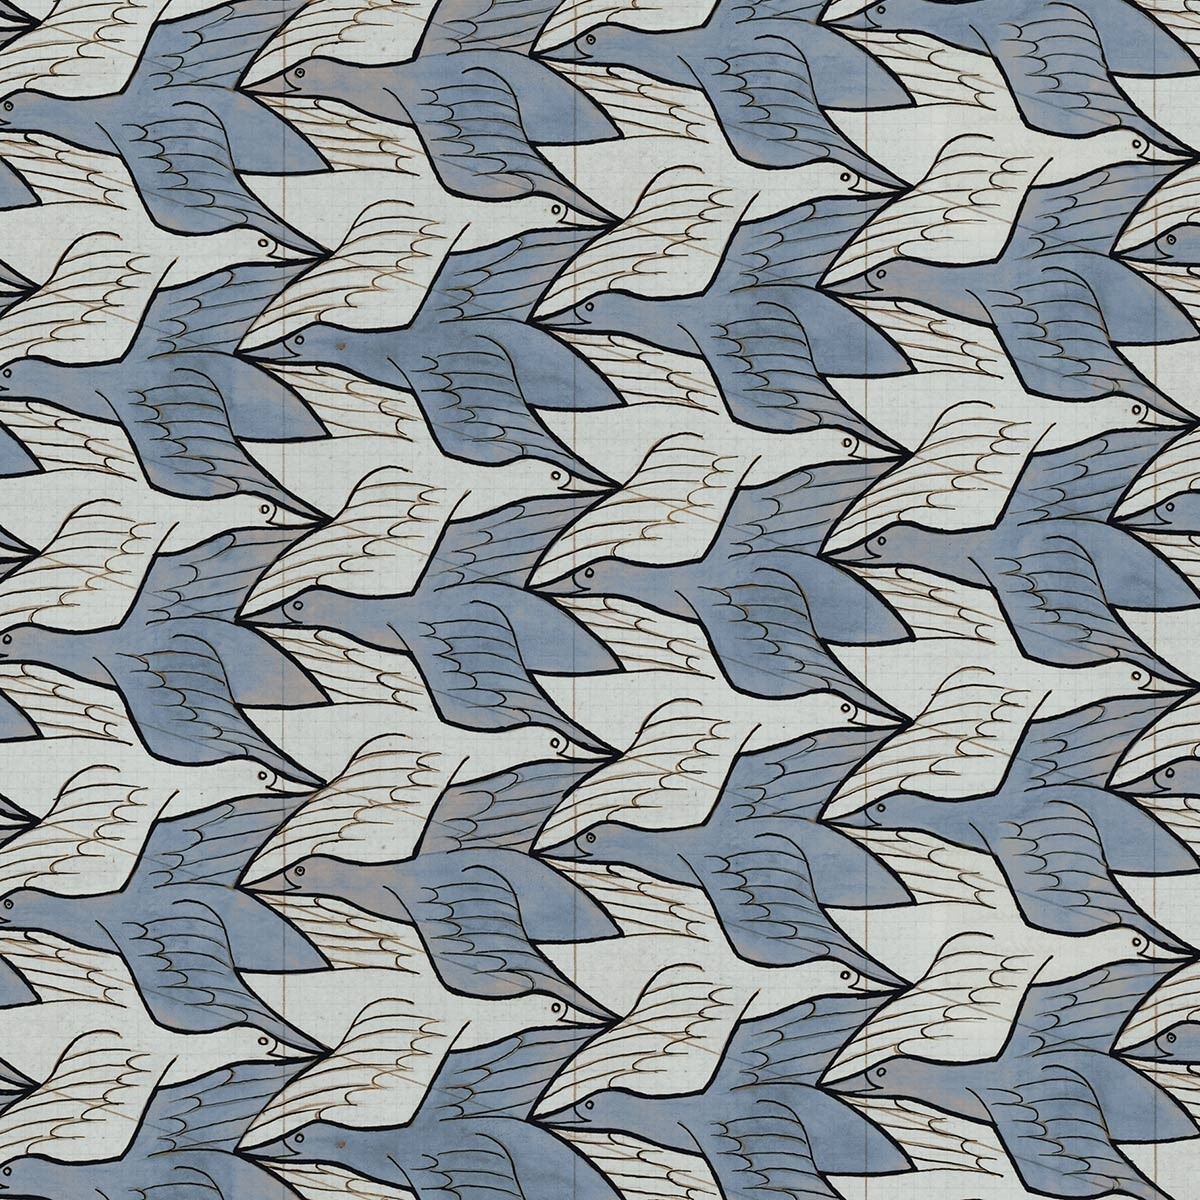
\includegraphics[scale=0.2, natwidth=1200, natheight=1200]{two-birds.jpg}
\end{center}

Inspired by this work, Ryan came up with Escher Sequence for 1D world:

\begin{itemize}
  \item Let $s$ be binary string (only contains $0$ and $1$)
  \item $s$ is an Escher Sequence if and only if $s = \t{flip(reverse(s))}$
  \item where \t{flip} changes all $0$ to $1$ (and vice versa),
  \item and \t{reverse} changes the order of string, for example: $0010$ to $0100$.
\end{itemize}

Now given an arbitrary binary string $s$,
Ryan wants to append minimum number of bits ($0$ or $1$) on end of $s$ to make it be an Escher Sequence.
